\documentclass{article}

\usepackage[english]{babel}
\usepackage{multirow}

\usepackage[letterpaper,top=2cm,bottom=2cm,left=3cm,right=3cm,marginparwidth=1.75cm]{geometry}
\usepackage{algorithm}
\usepackage{algpseudocode}
\usepackage{amsmath}
\usepackage{graphicx}
\usepackage{caption,subcaption}
\usepackage[colorlinks=true, allcolors=blue]{hyperref}

\title{Assignment 3 }
\author{Sherry Usman, Megan Mirnalini Sundaram R }

\begin{document}
\maketitle


\section*{Question 3.1}
\subsection*{1. Strategy for Calibration}
\begin{enumerate}
\item In order to effectively calibrate the set of images \emph{Cam01.tiff} and \emph{Cam02.tiff}  against the magnification of \emph{Cam03.tiff}, it is crucial to enhance their quality such that an accurate comparison can be made. One can do this by finding the edges of the image and then fine-tuning its intensities by thresholding. Additional morphological operations such as dilation and area opening can also be applied to enhance image quality and make the objects in the image stand out more. 
\item Then it is important to assess our \emph{a priori} knowledge of these images. Firstly, we know that the rulers depicted in the images are true to scale and not affected by distortion or skewness. Secondly, keeping the first point in mind, we know that the distance between two consecutive bars in the images is equal and represents 0.01 millimeters. Keeping this \emph{a priori} knowledge in mind we can effectively calibrate the images.  
\item Then it is important to find a common characteristic in both images that can be compared. In our case we chose the length between two distinct points lying on the ruler.
\item Once that is chosen it is important to find two distinct points that lie on the ruler in each image. This can be done by iterating through the image and finding the pixel with maximum intensity and/or minimum intensity. It should be noted that this technique does require further fine-tuning for point selection such that both points chosen lie on the ruler.
\item Then we can  measure the distance between them in pixels by using a simple euclidean distance formula and also the distance between in millimeters with the help of the ruler. 
\item Doing this for all three images will give us a table of distance values in pixels and millimeters. Then, given that the magnification of one image is known, simple ratios can be used to find the magnification of other images.
\end{enumerate}

\subsection*{2. Algorithm for Calibration}
The algorithm describes a detailed strategy to effectively calibrate images given that the magnification factor of one image is known.

\begin{algorithm}[h!]
\caption{Calibrate Images}\label{calibration_algo}
\begin{algorithmic}[1]
\Procedure{CalibrateImages}{$\text{images}$}
    \State $\text{distance\_list} \gets \text{empty list}$
    \For{$\text{image}$ \textbf{in} $\text{images}$}
        \State $image\_contrasted \gets \text{ContrastStretch}(image)$
        \State $image\_mag \gets \text{GradientMagnitude}(image\_contrasted)$
        \State $image\_dilated \gets \text{Dilation}(image\_mag)$
        \State $image\_opened \gets \text{AreaOpening}(image\_dilated)$
        \State $image\_labeled \gets \text{Label}(image\_opened)$
        \State $max \gets \text{FindMaxIntensityLoc}(image\_labeled)$
        \State $min \gets \text{FindMinIntensityLoc}(image\_labeled)$
        \State Adjust points to be on the ruler 
        \State $dist \gets \text{EuclideanDistance}(max, min)$
        \State Use the ruler to find the distance in millimeters between max and min
        \State $\text{distance\_list}.\text{append}(\text{dist})$
    \EndFor
    \State Use simple ratios of distance in pixels ${Dp_{1}}$ and ${Dp_{2}}$ and distance in millimeters $Dmm_{1}$ and $Dmm_{2}$ in simple ratios $\frac{\frac{Dp_{1}}{Dmm_{1}}}{\frac{Dp_{2}}{Dmm_{2}}}$ = $\frac{M_1}{M_2}$ to calculate the magnification $M_1$ and $M_2$ of other images 
    \State \textbf{return} $M_1$ and $M_2$
\EndProcedure
\end{algorithmic}
\end{algorithm}


\subsection*{3. Calibrated Images}
In order to accurately implement a calibration strategy it is important to remove noise and glare from the image. This can be done by using ContrastStretch provided in the dip.ContrastStretch function and adding an upper and lower bound to indicate the intensity scales you want to stretch the image to. In this case we found that a lower bound of 0.0 and an upper bound of 10.0 effectively removed enhanced our images and removed all noise. This can be shown in the figures below. \newline 


\begin{figure}[h!]
\centering
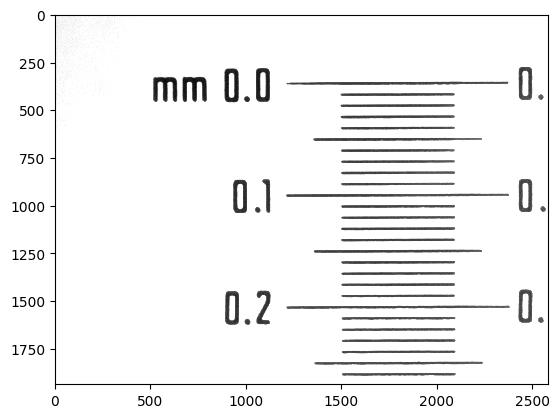
\includegraphics[width=0.4\linewidth]{Report/Images/contrasted_1.png}
\caption{\label{fig:cam1_contrasted}The figure shows image \emph{CamIm01.tif} after being contrast stretched.}
\end{figure}

\begin{figure}[h!]
\centering
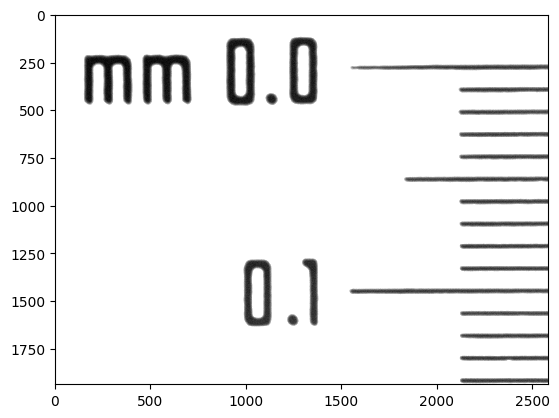
\includegraphics[width=0.4\linewidth]{Report/Images/contrasted_2.png}
\caption{\label{fig:cam2_contrasted}The figure shows image \emph{CamIm02.tif} after being contrast stretched.}
\end{figure}

\begin{figure}[h!]
\centering
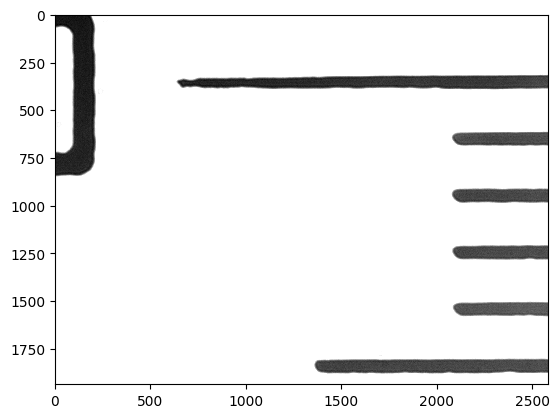
\includegraphics[width=0.4\linewidth]{Report/Images/contrasted_3.png}
\caption{\label{fig:cam3_contrasted}The figure shows image \emph{CamIm03.tif} after being contrast stretched.}
\end{figure}

Then as shown in the algorithm above it is important to apply additional morphological operations such as dilation and area opening to enhance image quality and make the edges of the ruler stand out more. \newline
Once that is done an iterative for-loop is used to find the maximum and minimum intensity and their specific locations. These locations are then adjusted to be on the ruler. This can be done by visualising the points on an image as shown in the figures below. \newline


\begin{tabular}{ |p{3cm}||p{3cm}|p{3cm}|p{3cm}|  }
 \hline
 \multicolumn{4}{|c|}{Image Measurements} \\
 \hline
Image & Distance between R and B (in pixels) &Distance between R and B (in mm) & Magnification\\
 \hline 
 image 1 & 1233  & 0.21 &  $M_{1}$\\ 
 image 2 & 720  &  0.06 &  $M_{2}$\\ 
 image 3 & 602  &  0.02 &  100\\ 
 \hline
\end{tabular}

\subsection*{4. Lens Magnification}

We first calculate the ratio R between distance between R and B in pixels and distance between R and B in millimeters. This equation is given below. 
\begin{equation}
R = \frac{\text{distance between R and B in pixels} }{\text{distance between R and B in mm}}
\end{equation}

Thus $R_{1}$ = $\frac{1233}{0.21}$ = 5871.4, $R_{2}$ = $\frac{720}{0.06}$ = 12000 and $R_{3}$ = $\frac{602}{0.02}$ = 30,100 $\approx$ 30,000. 
~\\ We do round off these values to remove any error. So if the magnification of image 3 is 100 with a ratio $R_{3}$ is 30,0000, then we can calculate the magnification of image 1 and 2 using simple ratios as shown below.

For image 1: 
\begin{equation}
\frac{30000}{100} = \frac{5871.4}{M_{1}}
\end{equation}
\begin{equation}
M_{1} = \frac{5871.4 \cdot 100}{30000}
\end{equation}
\begin{equation}
M_{1} = 20
\end{equation}

For image 2:
\begin{equation}
\frac{30000}{100} = \frac{12000}{M_{2}}
\end{equation}
\begin{equation}
M_{2} = \frac{12000 \cdot100}{30000}
\end{equation}
\begin{equation}
M_{2} = 40
\end{equation}

As shown in the calculations above, the magnification used by \emph{CamIm01.tiff} is 20 and the magnification used by \emph{CamIm02.tiff} is 40.
\clearpage
\section*{Question 3.2}
\subsection*{5. ICS Header and Details}
The below image shows the contents of the .ics file.
\begin{figure}[h!]
\centering
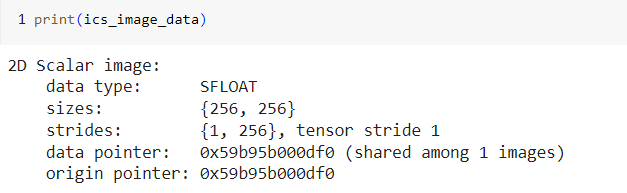
\includegraphics[width=0.8\linewidth]{Report/Images/ics_header_image.png}
\caption{\label{fig:ics_header_image}The figure shows the contents of the .ics file}
\end{figure}

The abbreviation \textbf{ICS} stands for \textbf{Image Cytometry Standard}. Customarily .ics images contain two different files: a .ics file which contains header information and .ids file which contains the data. In addition to image data it also contains the microscopic parameters describing the optics during image acquisition. \newline

As seen in Figure \ref{fig:ics_header_image}, the .ics file provides the specifications of the 2D image, including its data type SFLOAT, its size of 256 by 256 pixels and tensor stride of 1. This indicates that the im.ics is a two-dimensional image of 256 rows by 256 columns and filled with intensity values of type \textbf{floating point}. Furthermore, it has a tensor stride of 1 which means that the elements are stored continuously in memory along the first dimension in rows.  For this image the data pointer is 0x58fa14f30b20 which indicates that the image is stored at the location 0x58fa14f30b20 in memory. The origin pointer indicates where the image actually begins which is also 0x58fa14f30b20. \newline


\subsection*{6. Differences between .tif and .ics}
The below image shows the contents of the .tif file.
\begin{figure}[h!]
\centering
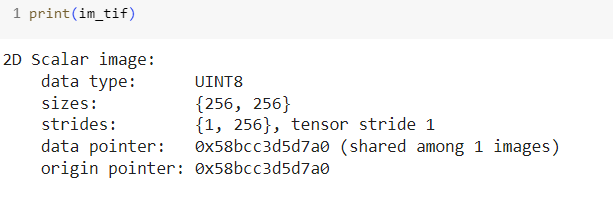
\includegraphics[width=0.8\linewidth]{Report/Images/tif_header_image.png}
\caption{\label{fig:tif_image}The figure shows the contents of the .tif file}
\end{figure}

As seen above, the .tif file provides the specifications of the 2D image, including its data type UINT8, its size of 256 by 256 pixels and tensor stride of 1. This indicates that the im.tif is a two-dimensional image of 256 rows by 256 columns and filled with intensity values of unsigned 8-bit integers. Furthermore, it has a tensor stride of 1 which means that the elements are stored continuously in memory along the first dimension in rows.  For this image the data pointer is 0x58fa14f30b20 which indicates that the image is stored at the location 0x58bcc3d5d7a0 in memory. The origin pointer indicates where the image actually begins which is also 0x58bcc3d5d7a0.

The main difference betweeen the .tif file and the .ics file lies in the datatype. While .ics stores the data in float values, .tif stores it as an integer. This is depicted in figure 6. A print of the first rows of both files shows that .ics file has a float datatype and the .tif file has integer datatype.  

\begin{figure}[h!]
\centering
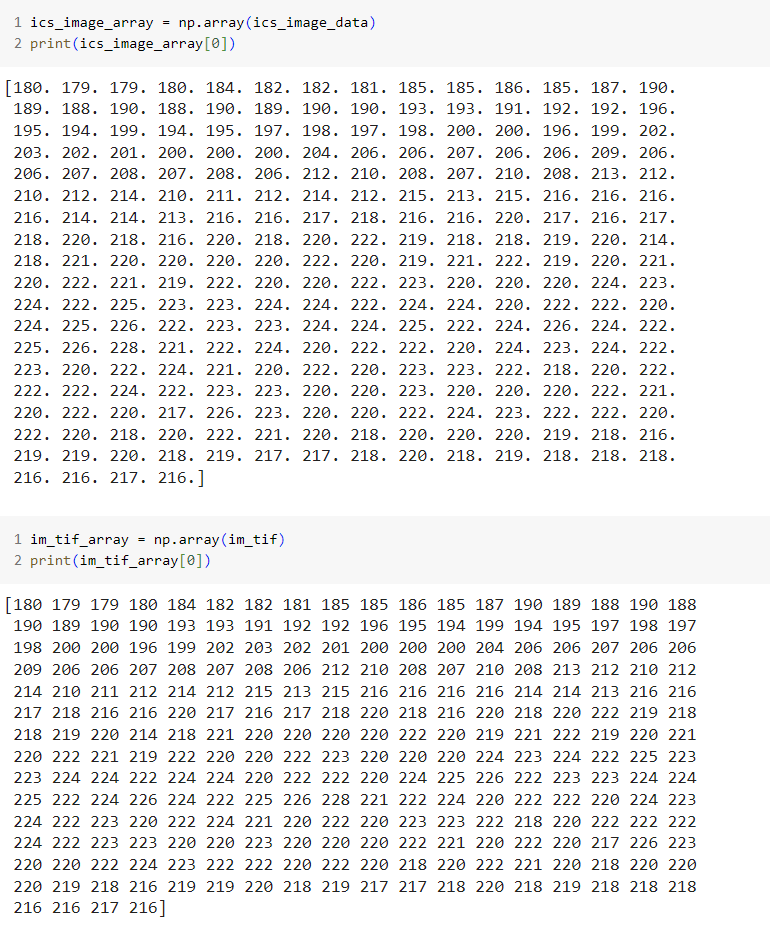
\includegraphics[width=0.8\linewidth]{Report/Images/ics_tif_datatype.png}
\caption{\label{fig:ics_tif_datatype_difference}The figure shows the first row of the .tif and .ics file}
\end{figure}

Furthermore, the sizes of the images are different. This is because .ics image stores single precision floating point values which are typically 32  bits each while the .tiff image stores unsigned 8 bit integers which are typically 8 bits each. 
\begin{figure}[h!]
\centering
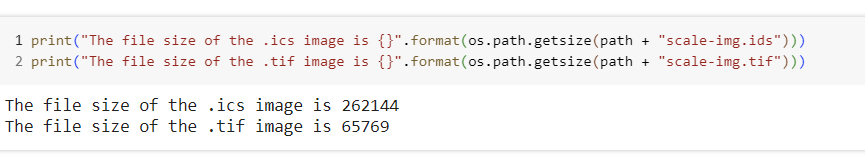
\includegraphics[width=0.8\linewidth]{Report/Images/filesize_difference.png}
\caption{\label{fig:ics_tif_filesize_difference}The figure shows the first row of the .tif and .ics file}
\end{figure}
As seen above, the file size of the .ics image is 262144, while the .tif image is 65769. 
$\frac{262144}{65769} = 3.98 \approx$ 4 , which shows the difference in the bytes. 
\clearpage
\section*{Question 3.3}
\subsection*{7. Strategy for preprocessing the images}
A first glance of existing images show that they suffer from uneven illumination and underexposure. A number of different mathematical morphological operations can be used to further enhance these images. Our strategy is to apply a morphological range operation with different kernel sizes, invert the result of the morphological range operation and then do a contrast stretch on the inverted image. The purpose of both operations is different: the morphological range operation implements a morphological edge detector based on the different parameters such as edge type and structuring element size. Contrast stretching on the other hand is an image enhancement technique that ensures that intensities are more evenly distributed along a histogram preventing underexposure or overexposure in this case. \newline \newline
For both these individual processes we intend to use different parameters. For example dip.ContrastStretch has parameters called upper bound and lower bound to stretch the image intensities to. Furthermore, dip.MorphologicalRange has parameters such as edgeType, object which we keep as default and structuring element which we vary. 

 \begin{algorithm}
\caption{Image Processing with Parameters}\label{image_processing_algo}
\begin{algorithmic}[1]
\Procedure{ImageProcessingWithParameters}{images, parameter1, parameter2, parameter3, parameter4}
    \State \textbf{Input:} 
        \Statex \hspace{\algorithmicindent} $images$: A set of input images
        \Statex \hspace{\algorithmicindent} $parameter1$: First an third parameter for contrast stretching operation
        \Statex \hspace{\algorithmicindent} $parameter2$: Second an fourth parameter for morphological range operation
    \State \textbf{Output:} 
        \Statex \hspace{\algorithmicindent} Processed images with contrast stretching and morphological range applied
    \ForAll{$image$ \textbf{in} $images$}
        \State Apply morphological range with $parameter1$: 
        \State \hspace{\algorithmicindent} \Call{MorphologicalRange}{$image$, $parameter2$}
        \State $inverted_image \gets \text{Invert}(morphed_image)$
        \State \hspace{\algorithmicindent} \Call{ContrastStretch}{$inverted_image$, $parameter2$}
        \State Save the processed images
    \EndFor
    \ForAll{$image$ \textbf{in} $images$}
        \State Apply morphological range with $parameter1$: 
        \State \hspace{\algorithmicindent} \Call{MorphologicalRange}{$image$, $parameter3$}
        \State $inverted_image \gets \text{Invert}(morphed_image)$
        \State \hspace{\algorithmicindent} \Call{ContrastStretch}{$inverted_image$, $parameter4$}
        \State Save the processed images
    \EndFor
    \State \textbf{return} Processed images
\EndProcedure
\end{algorithmic}
\end{algorithm}

\subsection*{8. Segmentation of the Images}
The images we produced after a morphological range and contrast stretch are shown in the appendix. In order to calibrate the images we applied further operations such as inversion, dilation and thresholding. This produced another set of images that we then labeled. From these images we can extract a number of image features such as center of gravity and maximum intensity location. From these datapoints we choose points whose distance can be measured using the scale via a continuous trial and error process. 
\begin{figure}[h!]
\centering
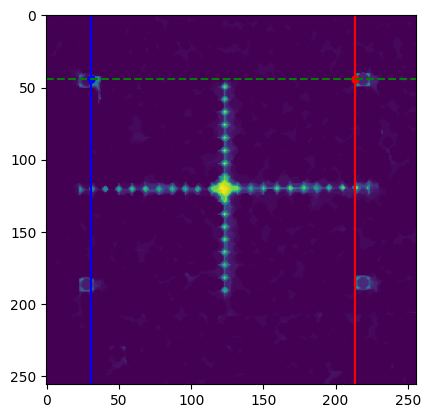
\includegraphics[width=0.4\linewidth]{Images/image_1_calculated.png}
\caption{\label{fig:background_correction}The figure shows image {im.tiff} after a morphological range of 5 and a contrast stretch of 30 was applied and two points were chosen and the distance between them was measured.}
\end{figure}

\begin{figure}[h!]
\centering
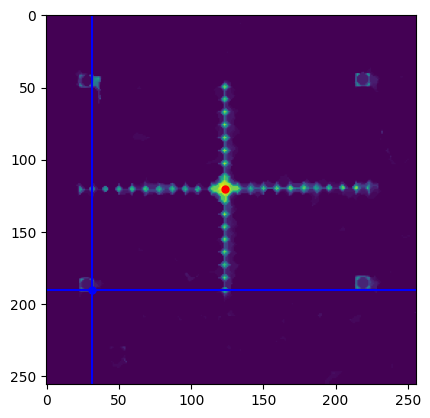
\includegraphics[width=0.4\linewidth]{Images/image2_calculated.png}
\caption{\label{fig:background_correction}The figure shows image {im.tiff} after a morphological range of 5 and constrast stretch of 15 was applied.}
\end{figure}

\begin{figure}[h!]
\centering
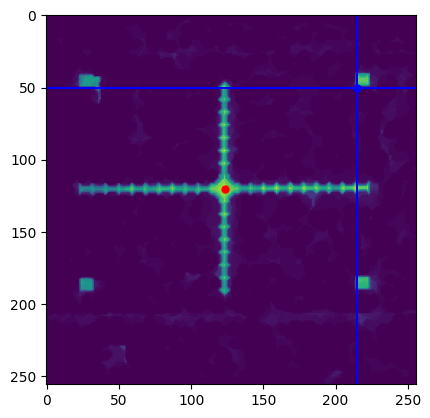
\includegraphics[width=0.4\linewidth]{Images/image_3.png}
\caption{\label{fig:background_correction}The figure shows image {im.tiff} after a morphological range of 10 and constrast stretch of 30 was applied.}
\end{figure}

\begin{figure}[h!]
\centering
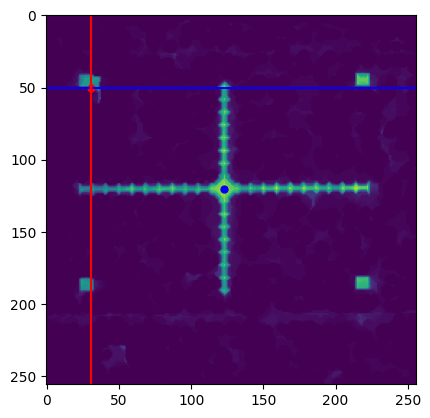
\includegraphics[width=0.4\linewidth]{Images/image_4.png}
\caption{\label{fig:background_correction}The figure shows image {im.tiff} after a morphological range of 10 and constrast stretch of 15 was applied.}
\end{figure}

After these results we can calculate the distance between the red and blue points using math.dist in python and using the ruler in the image to get the lengths in x and in y. Then the pythagoreas theorem can be used to calculate the diagonal distance between the red and blue points when they are diagonal. 

\begin{tabular}{ |p{3cm}||p{3cm}|p{3cm}|p{3cm}|  }
 \hline
 \multicolumn{4}{|c|}{Image Measurements} \\
 \hline
Image & Distance between R and B (in mm) &Distance between R and B (pi) & Magnification\\
 \hline 
 morph=5 cont=30 & 183.03  & 20 &  $PS_{1}$\\ 
 morph=5 cont=15  &  115.68 & 12.8  &  $PS_{2}$\\ 
 morph=10 cont=30 &  115.5 & 12.04 &  $PS_{2}$\\ 
 morph=10 cont=15 &  115.7 & 12.04 &  $PS_{2}$\\ 
 \hline
\end{tabular}

From this table we can calculate the pixel size in SI units (in this case milimeters). 
\begin{equation}
PS_{1} = \frac{183.03}{20}  = 9.15
\end{equation}

\begin{equation}
PS_{2} = \frac{115.68}{12.8}  = 9.03
\end{equation}

\begin{equation}
PS_{3} = \frac{115.5}{12.04}  = 9.59
\end{equation}

\begin{equation}
PS_{4} = \frac{115.7}{12.04}  = 9.6
\end{equation}

From our estimations we can see that a pixel holds an object of size approximately 9 by 9 mm.
\clearpage
\section*{Question 3.4}
\subsection*{9. Background Correction and Segmentation}
The below image shows image \emph{CamIm04.tif} after enhancement. 
\begin{figure}[h!]
\centering
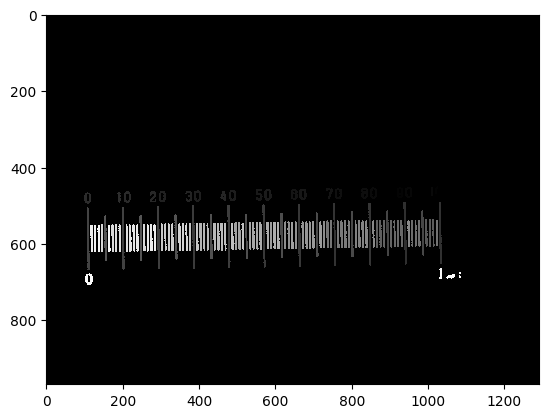
\includegraphics[width=0.8\linewidth]{Report/Images/a4_background_correction.png}
\caption{\label{fig:enhanced_cam4}The figure shows image {a4} after a number of enhancement operations were performed according to the strategy.}
\end{figure}

\subsubsection*{10. Pixel size of CamIn04}

\begin{tabular}{ |p{3cm}||p{3cm}|p{3cm}|p{3cm}| }
 \hline
 \multicolumn{4}{|c|}{Image Measurements} \\
 \hline
Image & Distance between R and B (in pixels) &Distance between R and B (in mm) & Magnification\\
 \hline 
 image 1 & 1233  & 0.21 &  20 \\
 image 2 & 720  &  0.06 &  40 \\
 image 3 & 602  &  0.02 &  100\\
 image 4 & 516.66 & 0.56 & $M_4$ \\
 \hline
\end{tabular}


Thus the ratio $R_4$ for image 4 is $\frac{516.66}{56}$ = 922.6. We can then calculate the magnification $M_4$ as follows:  

For image 1: 
\begin{equation}
\frac{30000}{100} = \frac{922.6}{M_{4}}
\end{equation}
\begin{equation}
M_{4} = \frac{922.6 x 100}{30000}
\end{equation}
\begin{equation}
M_{4} = 3.07 \approx 3
\end{equation}

Thus the magnification used by image 4 is 3. Since the magnification is smaller it is evident that is taken from a further distance than the images in question 1. 

\clearpage
\appendix
\section{Appendix}
\subsection*{Part 3.1}
\subsubsection*{Calibration}
The below figures were the by-product of the algorithm and was instrumental in calculating the magnification and distance. 
\begin{figure}[h!]
\centering
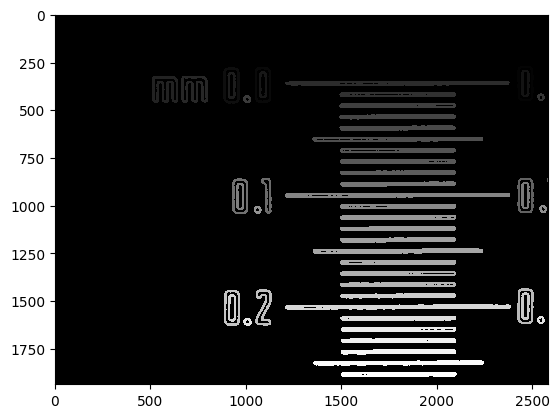
\includegraphics[width=0.4\textwidth]
{Report/Appendix_Images/processed_image_a1.png}
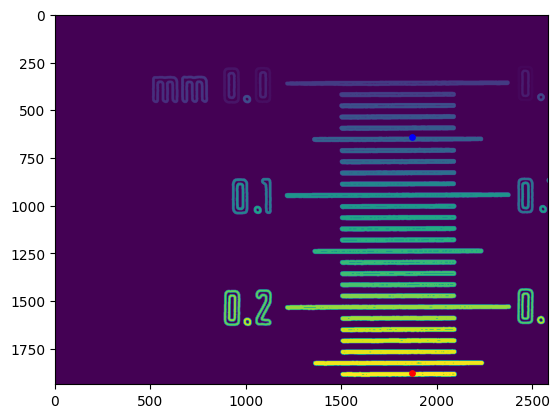
\includegraphics[width=0.4\textwidth]
{Report/Appendix_Images/processed_image_with_points_a1.png}
\caption{The first figure shows the calibrated image (the output from Algorithm \ref{calibration_algo} of \emph{CamIm01.tif} and the distance highlighted as two points} 
\label{A1_Calibration}
\end{figure}
\begin{figure}[h!]
\centering
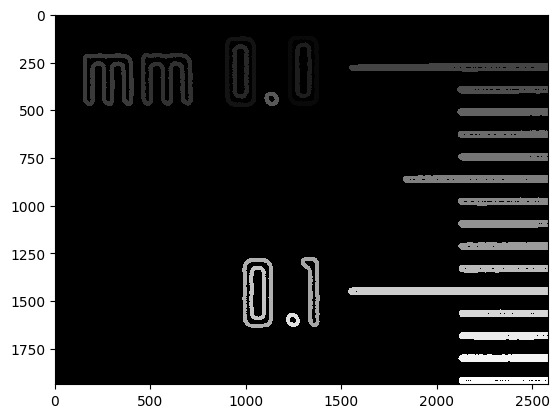
\includegraphics[width=0.4\textwidth]
{Report/Appendix_Images/processed_image_a2.png}
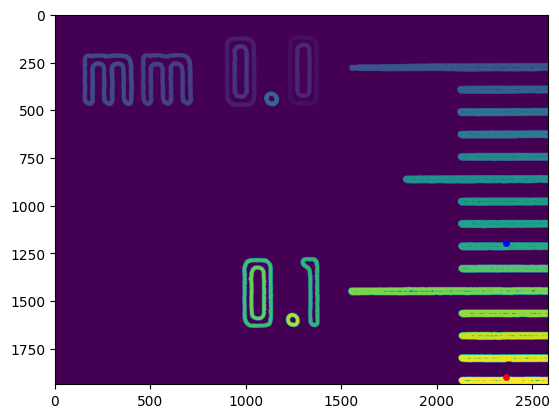
\includegraphics[width=0.4\textwidth]
{Report/Appendix_Images/processed_image_with_points_a2.png}
\caption{The first figure shows the calibrated image (the output from Algorithm \ref{calibration_algo} of \emph{CamIm02.tif} and the distance highlighted as two points} 
\label{A2_Calibration}
\end{figure}
\begin{figure}[h!]
\centering
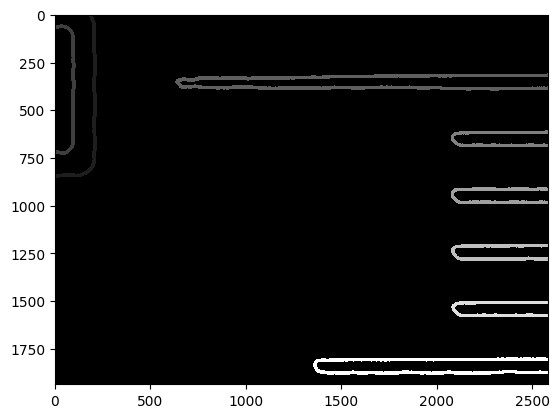
\includegraphics[width=0.4\textwidth]
{Report/Appendix_Images/processed_image_a3.png}
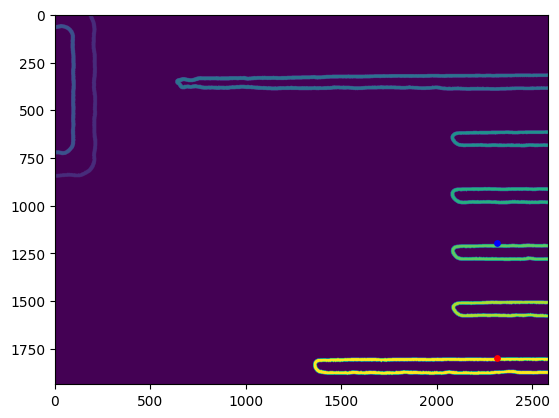
\includegraphics[width=0.4\textwidth]
{Report/Appendix_Images/processed_image_with_points_a3.png}
\caption{The first figure shows the calibrated image (the output from Algorithm \ref{calibration_algo} of \emph{CamIm03.tif} and the distance highlighted as two points} 
\label{A3_Calibration}
\end{figure}
\clearpage
\subsection*{Part 3.3}
The below set of images were generated after the initial set of segmentation and morphological operations. 
\begin{figure}[htb]
    \centering 
\begin{subfigure}{0.4\textwidth}
  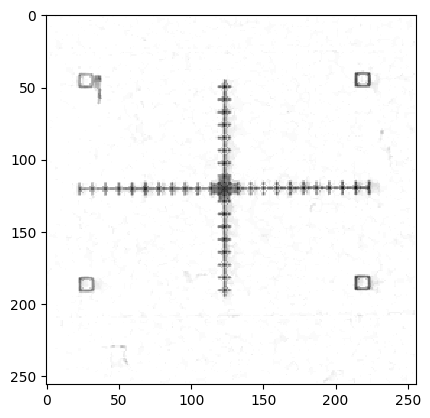
\includegraphics[width=\linewidth]{Report/Appendix_Images/im_tif_csr_5.png}
  \caption{\emph{im.tif} image after a morphological range of 5 and contrast stretch of 30 is applied. }
  \label{fig:im_tif_contrast_30}
\end{subfigure}\hfil 
\begin{subfigure}{0.4\textwidth}
  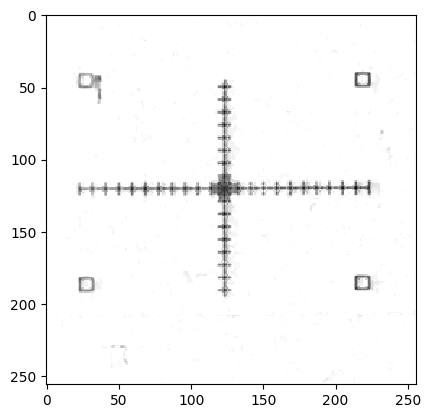
\includegraphics[width=\linewidth]{Report/Appendix_Images/im_tif_csr_5_15.png}
  \caption{\emph{im.tif } image after a morphological range of 5 and contrast stretch of 15 is applied.}
  \label{fig:im_tif_contrast_15}
\end{subfigure}\hfil 
\begin{subfigure}{0.4\textwidth}
  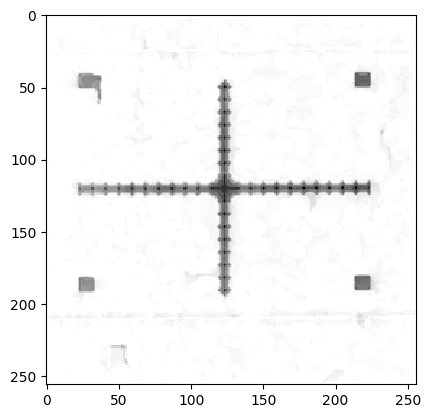
\includegraphics[width=\linewidth]{Report/Appendix_Images/im_tif_csr_10.png}
  \caption{\emph{im.tif } image after a morphological range of 10 and contrast stretch of 30 is applied.}
  \label{fig:im_tif_contrast_30}
\end{subfigure}
\medskip
\begin{subfigure}{0.4\textwidth}
  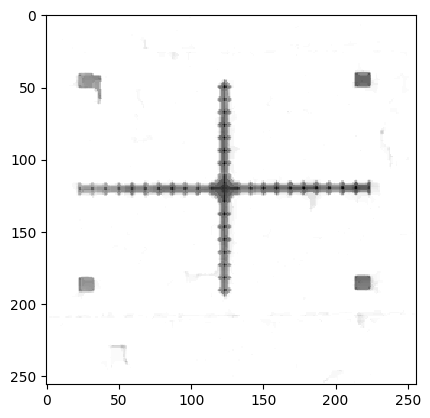
\includegraphics[width=\linewidth]{Report/Appendix_Images/im_tif_csr_10_15.png}
  \caption{\emph{im.tif} image after a morphological range of 10 and contrast stretch of 15 is applied.}
  \label{fig:4}
\end{subfigure}\hfil 

\end{figure}

\begin{figure}[htb]
    \centering 
\begin{subfigure}{0.4\textwidth}
  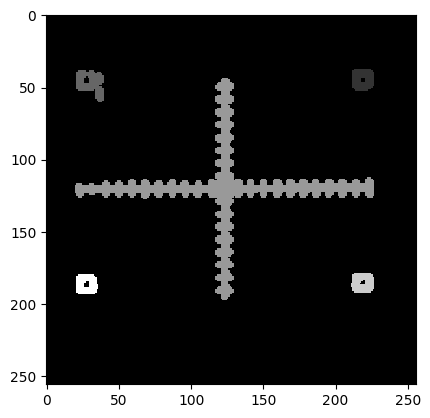
\includegraphics[width=\linewidth]{Report/Appendix_Images/black1.png}
  \caption{The inverse of \emph{im.tif} image after a morphological range of 5 and contrast stretch of 30 is applied labelled. }
  \label{fig:1}
\end{subfigure}\hfil 
\begin{subfigure}{0.4\textwidth}
  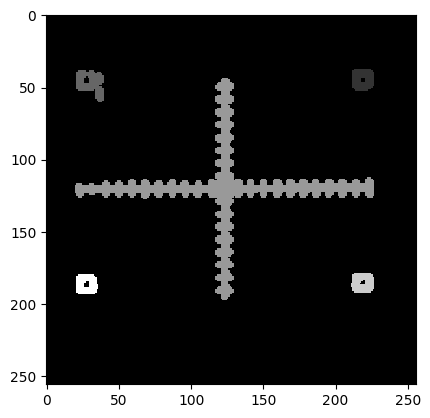
\includegraphics[width=\linewidth]{Report/Appendix_Images/black2.png}
  \caption{The inverse of \emph{im.tif} image after a morphological range of 5 and contrast stretch of 15 is applied labelled.}
  \label{fig:2}
\end{subfigure}\hfil 
\begin{subfigure}{0.4\textwidth}
  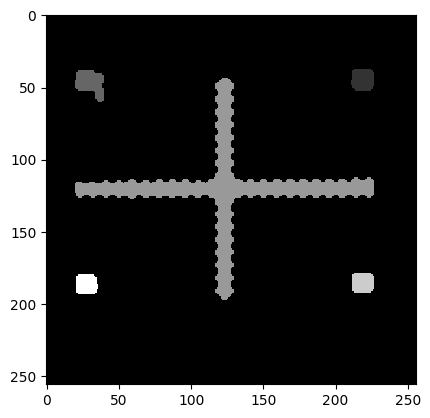
\includegraphics[width=\linewidth]{Report/Appendix_Images/black3.png}
  \caption{The inverse of \emph{im.tif} image after a morphological range of 10 and contrast stretch of 30 is applied labelled.}
  \label{fig:3}
\end{subfigure}
\medskip
\begin{subfigure}{0.4\textwidth}
  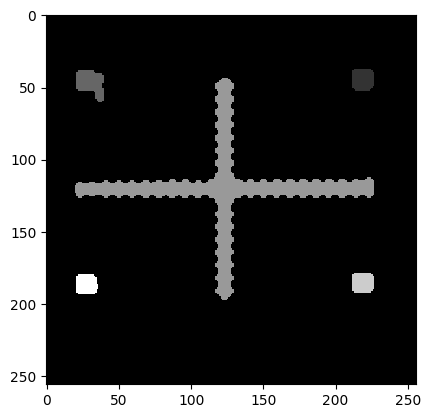
\includegraphics[width=\linewidth]{Report/Appendix_Images/black4.png}
  \caption{The inverse of \emph{im.tif} image after a morphological range of 10 and contrast stretch of 15 is applied labelled.}
  \label{fig:4}
\end{subfigure}\hfil 
\end{figure}
\clearpage
\subsection*{Part 3.4}
The below set of images were the byproducts of background correction and segmentation on \emph{CamIm04.tif}

\begin{figure}[h!]
  \centering
  \begin{subfigure}{0.4\textwidth}
    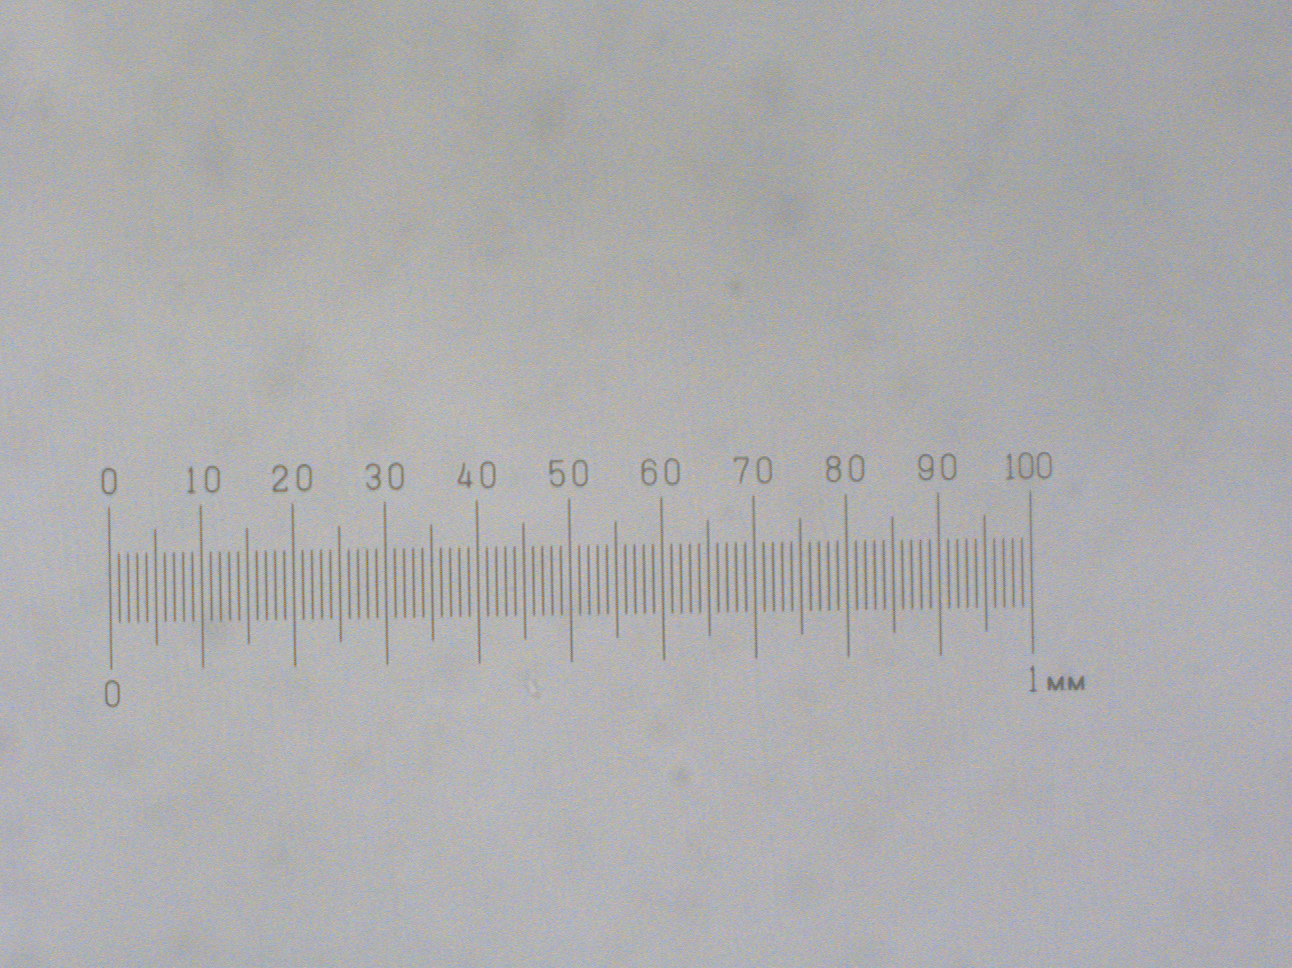
\includegraphics[width=\linewidth]{Report/Appendix_Images/a4_original.png}
    \caption{\emph{CamIm04.tif} - the original image}
  \end{subfigure}
  \hfill
  \begin{subfigure}{0.4\textwidth}
    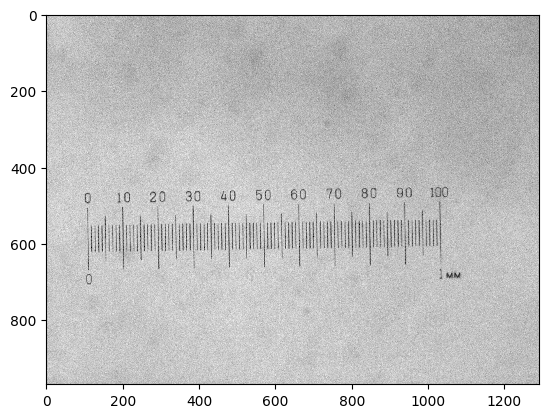
\includegraphics[width=\linewidth]{Report/Appendix_Images/a4_grey_image.png}
    \caption{Grey Value Thresholding applied to it}
  \end{subfigure}

  \begin{subfigure}{0.4\textwidth}
    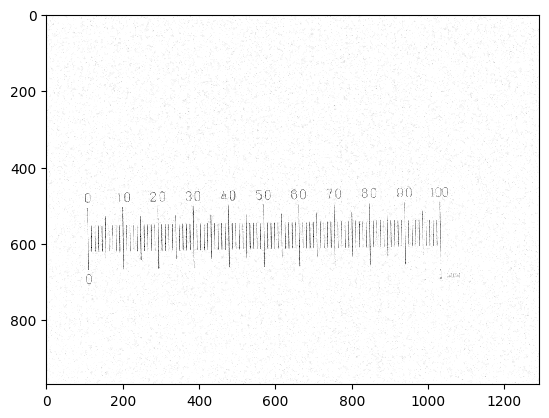
\includegraphics[width=\linewidth]{Report/Appendix_Images/a4_contrast_stretched.png}
    \caption{The contrast-stretched image}
  \end{subfigure}
  \hfill
  \begin{subfigure}{0.4\textwidth}
    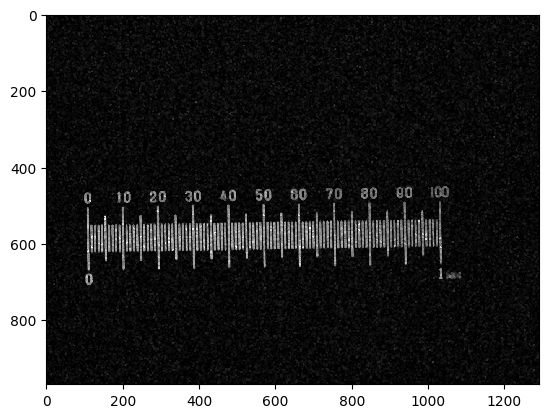
\includegraphics[width=\linewidth]{Report/Appendix_Images/a4_dilated.png}
    \caption{The image after inversion and dilation}
  \end{subfigure}

  \begin{subfigure}{0.4\textwidth}
    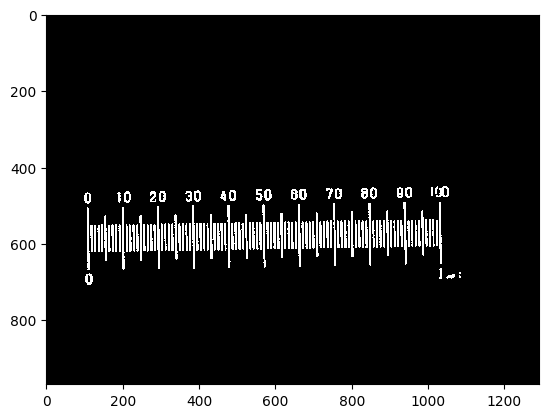
\includegraphics[width=\linewidth]{Report/Appendix_Images/a4_thresholded.png}
    \caption{The image after isodata thresholding}
  \end{subfigure}
  \hfill
  \begin{subfigure}{0.4\textwidth}
    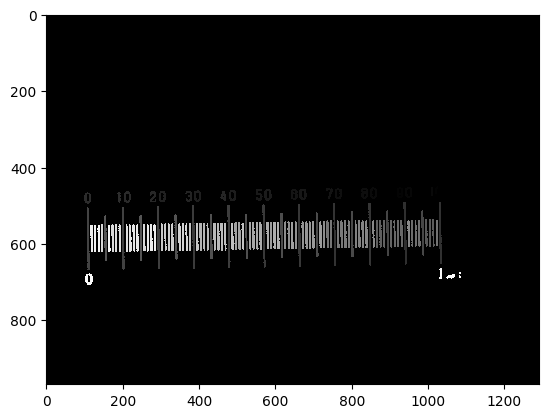
\includegraphics[width=\linewidth]{Report/Images/a4_background_correction.png}
    \caption{The background corrected final image}
  \end{subfigure}
\end{figure}
\end{document}
